\section*{This is how we go about it}
\begin{itemize}
\item First of all, let's take a look at a possible spliting. For this we have to make sure that all possible meaningful diagrams have been considered. 
\begin{figure}[h!]
\centering
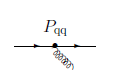
\includegraphics[scale=0.7]{images/Intro/pqq.png}
\end{figure}

\begin{figure}[h!]
\centering
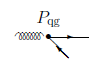
\includegraphics[scale=0.7]{images/Intro/pqg.png}
\end{figure}
(b) A daughter quark from a parent gluon which splits into a
quark-antiquark pair. Here no singularity develops since daughter
and parent can always be distinguished.
\begin{figure}[h!]
\centering
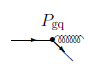
\includegraphics[scale=0.7]{images/Intro/pgq.png}
\end{figure}
(c) A daughter gluon from a quark parent. Also here no singularity.

\begin{figure}[h!]
\centering
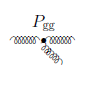
\includegraphics[scale=0.7]{images/Intro/pgg.png}
\end{figure}
(d) A daughter gluon from a parent gluon. Like in q ! qg a

singularity develops in the soft limit $ (1-z) \rightarrow 0  $.
\item The square matrix element is a complex number and therefore:
\item we have to keep all indices as they are defined at $M_1$ and $M_2$. This is very important for the calculation of the interference term in order to get a meaningful result.
\item In the case of the gluon loop, you have to add the corresponding ghost diagram.
\item for all parts of the matrix element, use the parametrisation and the recipe for sending the kinematics from the last section.
After the addition of all terms we get all singularities (soft and collinear). 
\item To determine whether everything was calculated correctly, one goes to the collinear limits, so to speak for y, because here one has to get the Alterali-Parisi splitting function known in the parton shower
\end{itemize}